\documentclass[9pt,a4paper]{extarticle}

% ======================
% Codificação, idioma e layout
% ======================
\usepackage[T1]{fontenc}
\usepackage[utf8]{inputenc}
\usepackage[brazil]{babel}
\usepackage{geometry}
\geometry{margin=2cm}
\usepackage{parskip}
\usepackage{setspace}
\usepackage{microtype}

% ======================
% Matemática e símbolos
% ======================
\usepackage{amsmath, amssymb, amsthm}

% ======================
% Figuras, tabelas e cores
% ======================
\usepackage{graphicx}
\usepackage{float}
\usepackage{caption}
\usepackage{subcaption}
\usepackage{xcolor}
\usepackage{booktabs}
\usepackage{array}
\usepackage{tabularx}

% ======================
% Listas e hyperlinks
% ======================
\usepackage{enumitem}
\setlist{nosep}
\usepackage{hyperref}
\hypersetup{
  colorlinks=true,
  urlcolor=blue,
  linkcolor=blue
}

% ======================
% Código fonte (UTF-8 seguro)
% ======================
\usepackage{listings}
\definecolor{codebg}{rgb}{0.95,0.95,0.95}
\lstset{
  language=Python,
  backgroundcolor=\color{codebg},
  basicstyle=\ttfamily\footnotesize,
  keywordstyle=\color{blue},
  commentstyle=\color{gray},
  stringstyle=\color{red!70!black},
  showstringspaces=false,
  frame=single,
  breaklines=true,
  extendedchars=true,
  inputencoding=utf8,
  literate={á}{{\'a}}1 {ã}{{\~a}}1 {â}{{\^a}}1 {é}{{\'e}}1 {ê}{{\^e}}1
           {í}{{\'i}}1 {ó}{{\'o}}1 {õ}{{\~o}}1 {ô}{{\^o}}1 {ú}{{\'u}}1
           {ç}{{\c c}}1 {Á}{{\'A}}1 {Ã}{{\~A}}1 {Â}{{\^A}}1 {É}{{\'E}}1
           {Ê}{{\^E}}1 {Í}{{\'I}}1 {Ó}{{\'O}}1 {Õ}{{\~O}}1 {Ô}{{\^O}}1
           {Ú}{{\'U}}1 {Ç}{{\c C}}1
}

% ======================
% Macros
% ======================
\newcommand{\Astar}{A\textsuperscript{*}}

% ======================
% Dados do documento
% ======================
\title{Roteiro de Aula 3 -- Busca Informada (Cap. 3.5.4 e 3.6, Poole \& Mackworth, AIFCA 3e)}
\author{Disciplina: BCC740 -- Inteligência Artificial}
\date{\today}

\begin{document}
\maketitle

\section*{Sumário da Aula}
\begin{enumerate}
  \item 3.6 \textbf{Busca Informada (Heurística): motivação e definições}
  \item 3.5.4 \textbf{Lowest-Cost-First (Uniform-Cost) Search} \emph{[ponte para \Astar]}
  \item \textbf{Heuristic Depth-First} e \textbf{Greedy Best-First}
  \item 3.6.1 \textbf{Busca \Astar}
  \item 3.6.2 \textbf{Branch and Bound}
  \item 3.6.3 \textbf{Construção de Heurísticas}
\end{enumerate}

\section{Pré-requistos}

% ===============================================================
\subsection{Estruturas de Dados: Filas de Prioridade e Heaps}
% ===============================================================

Os algoritmos \textbf{Uniform-Cost}, \textbf{A\Astar}, e outras variantes de busca informada
utilizam uma \textbf{fronteira} (ou \textit{open list}) organizada como uma
\textbf{fila de prioridade}.  
O objetivo é sempre expandir primeiro o nó com menor valor de custo
(ou estimativa de custo).

\subsection*{Heaps: Estrutura de Dados para Fila de Prioridade}

Uma implementação eficiente de fila de prioridade é o \textbf{heap binário}.
Um heap é uma estrutura de árvore quase completa que mantém a seguinte propriedade:

\begin{quote}
  Para cada nó, o valor armazenado é menor ou igual (em um \textit{min-heap})
  ou maior ou igual (em um \textit{max-heap}) que o valor dos filhos.
\end{quote}

Isso garante que o elemento de menor valor esteja sempre na raiz, o que permite:
\begin{itemize}
  \item Inserção de um novo elemento em tempo $O(\log n)$;
  \item Remoção (ou acesso) ao elemento mínimo em tempo $O(\log n)$;
  \item Verificação do mínimo em tempo $O(1)$.
\end{itemize}

\subsection*{Heap em Python}

O módulo \texttt{heapq} da biblioteca padrão implementa um \textit{min-heap} sobre listas.
Os elementos inseridos devem ser \emph{tuplas} ou objetos comparáveis,
de modo que a comparação seja feita pelo primeiro item da tupla.

\begin{lstlisting}
import heapq

# Exemplo básico:
fronteira = []
heapq.heappush(fronteira, (3, "C"))
heapq.heappush(fronteira, (1, "A"))
heapq.heappush(fronteira, (2, "B"))

# Removendo o menor elemento
_, estado = heapq.heappop(fronteira)
print(estado)  # Saída: "A"
\end{lstlisting}

Na implementação de busca, as tuplas costumam conter:
\[
(\text{prioridade}, \text{desempate}, \text{nó})
\]
onde \texttt{prioridade} é o valor de custo $g(n)$ (UCS) ou $f(n)=g(n)+h(n)$ (A\Astar).

\paragraph{Resumo:}
\begin{itemize}
  \item \texttt{heapq.heappush(heap, elemento)} insere com custo $O(\log n)$;
  \item \texttt{heapq.heappop(heap)} remove o menor elemento com custo $O(\log n)$;
  \item Heaps são cruciais para manter a eficiência de UCS e A\Astar, evitando varreduras lineares.
\end{itemize}


% ===============================================================
\section{Busca Informada: Motivação}
% ===============================================================

As estratégias não informadas (BFS, DFS, UCS) não consideram diretamente quão perto um estado está da meta.
A \textbf{busca informada} utiliza uma \textbf{função heurística} $h(n)\!\ge\!0$ que estima o custo do melhor caminho de $n$ até a meta.

\subsection*{Definições}
$h$ é \textbf{admissível} se $h(n)\le h^*(n)$, onde $h^*(n)$ é o custo real mínimo de $n$ à meta.
Quanto melhor a qualidade de $h$, mais a busca é guiada para regiões promissoras do espaço.

\paragraph{Derivação de heurísticas (ideia):} resolver um \emph{problema simplificado} e usar seu custo como estimativa (linha reta em rotas; Manhattan no 8-puzzle; bancos de padrões etc.).

% ===============================================================
\section{3.5.4 Lowest-Cost-First (Uniform-Cost) Search}
% ===============================================================

Em muitos domínios, os arcos têm \textbf{custos não unitários} e o objetivo é \textbf{minimizar o custo total} do caminho até a meta.
A \textbf{lowest-cost-first search} (ou \textbf{uniform-cost search}, UCS) expande sempre o caminho de \textbf{menor custo acumulado} $g(p)$ na fronteira.

\subsection*{Ideia e Implementação}
\begin{itemize}
  \item Trate a \textbf{fronteira} como uma \textbf{fila de prioridade} ordenada por $g(p)$.
  \item Ao expandir, gere sucessores com seus custos atualizados e reinsira na fronteira.
  \item Quebra de empates pode seguir ordem FIFO, menor profundidade, ou mesmo menor $h$ (se disponível) apenas como \emph{desempate} --- não altera a otimalidade de UCS.
\end{itemize}

\begin{lstlisting}
import heapq

class Node:
    __slots__ = ("state","parent","action","g","depth")
    def __init__(self, state, parent=None, action=None, g=0.0):
        self.state  = state
        self.parent = parent
        self.action = action
        self.g      = g
        self.depth  = 0 if parent is None else parent.depth + 1

def solution(n):
    path = []
    while n and n.parent is not None:
        path.append(n.action)
        n = n.parent
    return list(reversed(path))

def uniform_cost_search(s0, is_goal, successors):
    """Retorna a sequência de ações de menor custo (se existir)."""
    start = Node(s0, None, None, g=0.0)
    frontier = [(0.0, id(start), start)]   # (g, tie, node)
    best_g = {}                            # melhor custo por estado

    while frontier:
        g, _, node = heapq.heappop(frontier)
        if is_goal(node.state):
            return solution(node)
        # poda por custo já conhecido
        if node.state in best_g and best_g[node.state] <= g:
            continue
        best_g[node.state] = g
        for (a, s_next, cost) in successors(node.state):
            g_next = g + float(cost)       # custos de arco > 0
            child = Node(s_next, node, a, g_next)
            heapq.heappush(frontier, (g_next, id(child), child))
    return None
\end{lstlisting}

\subsection*{Corretude e Condições Suficientes}

Se (i) o fator de ramificação é finito e (ii) todos os custos de arco são
\textbf{estritamente positivos} ($\ge \epsilon > 0$), então a
\textbf{busca de custo uniforme (UCS)} é \textbf{completa} e
\textbf{ótima}.  
Em particular, o \emph{primeiro} caminho-meta removido da fronteira
é aquele de menor custo total $g(p)$ — logo, a solução retornada é ótima.

\paragraph{Racional:}
a UCS expande caminhos a partir do nó inicial em \emph{ordem crescente de custo acumulado}.
Como os custos de arco são positivos, os valores de $g(p)$ nunca diminuem ao longo do processo.
Assim, nenhum caminho mais barato pode ser descoberto após a expansão de um mais caro:
se existisse uma solução de custo menor que a primeira encontrada, ela teria sido expandida
antes da solução atual.

\paragraph{Importância do limite inferior ($\epsilon>0$):}
A exigência de custos de arco \emph{limitados inferiormente}
— isto é, todos os arcos possuem custo maior que uma constante positiva —
garante que o algoritmo não ficará preso em caminhos infinitos de custo finito.
Com esse limite, a UCS sempre encontrará uma solução (se existir) em grafos com
fator de ramificação finito.

\paragraph{Nota (paradoxo de Zeno):}
Sem o limite inferior $\epsilon$, podem existir caminhos infinitos
cujo custo total permanece finito.
Por exemplo, considere uma sequência de nós
$n_0, n_1, n_2, \dots$
com arcos $\langle n_{i-1}, n_i \rangle$ de custo $1/2^i$.
Cada caminho finito
$\langle n_0, n_1, \dots, n_k \rangle$
terá custo menor que $1$,
mas a soma total converge para $1$.
Se existir um arco direto de $n_0$ para o nó-meta com custo exatamente $1$,
a UCS nunca o expandirá,
pois continuará gerando extensões infinitas do caminho parcial de custo ligeiramente menor que $1$.
Essa situação é uma analogia moderna ao \emph{paradoxo de Zeno} descrito por Aristóteles há mais de dois milênios.


\subsection*{Complexidade (pior caso)}
Se $c$ é o custo da solução ótima e $k=c/\epsilon$, a busca pode gerar até $O(b^{k})$ caminhos de comprimento $\le k$, resultando em \textbf{tempo} e \textbf{espaço} $O(k\,b^{k})$.

\paragraph{Ponte para \Astar}
UCS é um caso particular de \Astar\ quando $h(n)\equiv 0$, logo $f(n)=g(n)$.
Essa visão unifica UCS e \Astar\ sob a mesma política de fila de prioridade.

% ===============================================================
\section{Heuristic Depth-First e Greedy Best-First}
% ===============================================================

\subsection*{Heuristic Depth-First Search}
Ordena vizinhos por $h(n)$, expandindo o mais promissor primeiro. Não garante completude nem otimalidade.

\subsection*{Greedy Best-First Search}
Seleciona sempre o nó com menor $h(n)$ na fronteira ($f(n)=h(n)$). Pode ser rápido, mas é míope e pode ciclar.

\begin{lstlisting}
def greedy_best_first_search(s0, is_goal, successors, h):
    from heapq import heappush, heappop
    frontier = []
    heappush(frontier, (h(s0), Node(s0)))
    explored = set()
    while frontier:
        _, node = heappop(frontier)
        if is_goal(node.state):
            return solution(node)
        explored.add(node.state)
        for (a, s_next, cost) in successors(node.state):
            if s_next not in explored:
                heappush(frontier, (h(s_next), Node(s_next, node, a)))
    return None
\end{lstlisting}

% ===============================================================
\section{Busca \Astar}
% ===============================================================

A \Astar\ usa $f(n)=g(n)+h(n)$, combinando custo acumulado e heurística.
Se $h$ é admissível e os custos de arco são $\ge \epsilon>0$, \Astar\ é \textbf{completa} e \textbf{ótima}.

\begin{lstlisting}
def a_star_search(s0, is_goal, successors, h):
    import heapq
    start = Node(s0, None, None, 0.0)
    frontier = [(h(s0), id(start), start)]
    best_g = {}
    while frontier:
        f, _, node = heapq.heappop(frontier)
        if is_goal(node.state):
            return solution(node)
        if node.state in best_g and best_g[node.state] <= node.g:
            continue
        best_g[node.state] = node.g
        for (a, s_next, cost) in successors(node.state):
            g_next = node.g + float(cost)
            heapq.heappush(frontier, (g_next + h(s_next),
                                      id(node) ^ hash(s_next),
                                      Node(s_next, node, a, g_next)))
    return None
\end{lstlisting}

\paragraph{Intuição:}
\[
\text{start} \xrightarrow{g(n)} n \xrightarrow{h(n)} \text{goal}
\quad \Rightarrow \quad f(n) = g(n) + h(n).
\]

\paragraph{Admissibilidade (esboço):}
Com $b<\infty$, custos $\ge \epsilon>0$ e $h$ admissível, a primeira solução retornada por \Astar\ é ótima.

% ===============================================================
\subsection*{Consistência (Monotonicidade) da Heurística}
% ===============================================================

Além de ser \textbf{admissível}, uma heurística pode também satisfazer uma condição mais forte,
chamada de \textbf{consistência} (ou \textbf{monotonicidade}):

\[
  h(n) \le c(n, n') + h(n')
\]
para todo arco $(n, n')$ com custo $c(n, n')$.

\paragraph{Intuição:}
a estimativa nunca “salta” mais do que o custo real entre dois estados adjacentes.
Isso implica que a função $f(n)=g(n)+h(n)$ é \emph{não decrescente}
ao longo de qualquer caminho — o que permite reusar nós sem precisar reabrir a fronteira.

\paragraph{Relações Importantes:}
\begin{itemize}
  \item Toda heurística consistente é também admissível.
  \item O inverso nem sempre é verdadeiro.
  \item Se $h$ é consistente, o A\Astar\ não precisa reexpandir nós: o primeiro custo encontrado para um estado é o menor possível.
\end{itemize}

% ===============================================================
\subsection*{Prova (Esboço) de Otimalidade do \Astar}
% ===============================================================

A seguir apresenta-se uma visão resumida da demonstração de que o \Astar,
com $h$ admissível e custos positivos, é \textbf{ótimo}.

\paragraph{Hipóteses:}
\begin{enumerate}
  \item Custos de arco $c(n,n') \ge \epsilon > 0$.
  \item Fator de ramificação $b < \infty$.
  \item Heurística $h$ é admissível, ou seja, $h(n) \le h^*(n)$.
\end{enumerate}

\paragraph{Ideia da prova:}
Seja $G_1$ o primeiro nó-meta removido da fronteira pelo \Astar.
Suponha, por contradição, que existe outro caminho $P^*$ de custo menor ($C^* < g(G_1)$).
Como $h$ é admissível,
cada nó $n$ em $P^*$ teria $f(n) = g(n)+h(n) \le C^*$,
logo todos esses nós teriam prioridade menor que $G_1$ na fila de prioridade.
Mas então o \Astar\ teria expandido $P^*$ antes de $G_1$, o que é uma contradição.
Portanto, $g(G_1)=C^*$ e a solução é ótima.

\paragraph{Visualização:}
\begin{figure}[H]
  \centering
  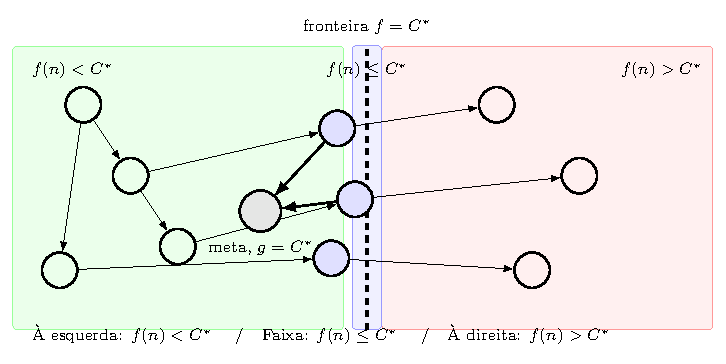
\includegraphics[width=.7\linewidth]{figure1.pdf}
  \caption{Esboço visual: os nós à esquerda da fronteira possuem $f(n) < C^*$,
  os da fronteira têm $f(n) \le C^*$ e os à direita $f(n) > C^*$.
  O primeiro nó-meta removido terá custo ótimo $C^*$.}
\end{figure}

\paragraph{Consequência prática:}
A\Astar\ é:
\begin{itemize}
  \item \textbf{Completa}, se há limite inferior $\epsilon$ no custo dos arcos.
  \item \textbf{Ótima}, se $h$ é admissível (ou consistente).
\end{itemize}

% ===============================================================
\section{Branch and Bound}
% ===============================================================

Combina \textbf{DFS} com um \textbf{limite (bound)}: poda caminhos com $g(n)+h(n)$ não menor que o melhor custo encontrado.
Gera soluções cada vez melhores e retorna a ótima no final; economiza memória comparado a expandir em largura.

% ===============================================================
\section{Construção de Heurísticas}
% ===============================================================

Heurísticas admissíveis via \emph{problema simplificado}:
\begin{itemize}
  \item Rotas: distância em linha reta (Euclidiana).
  \item 8-puzzle: peças fora do lugar; soma de distâncias Manhattan.
  \item Entrega de pacotes: maior distância necessária entre coletas/destinos.
\end{itemize}

\paragraph{Pattern Databases:} pré-compute soluções de subproblemas e armazene para consultas rápidas de $h$.

% ===============================================================
\section{Resumo Comparativo}
% ===============================================================

\begin{table}[H]
\centering
\small
\setlength{\tabcolsep}{4pt}
\renewcommand{\arraystretch}{1.2}
\begin{tabular}{@{}lccccp{5.2cm}@{}}
\toprule
\textbf{Método} & \textbf{Usa $g(n)$} & \textbf{Usa $h(n)$} & \textbf{Completo} & \textbf{Ótimo} & \textbf{Observações} \\
\midrule
UCS (Lowest-Cost-First) & Sim & Não & Sim ($\epsilon>0$) & Sim & Caso especial de \Astar\ com $h\equiv 0$. \\
Greedy Best-First       & Não & Sim & Não               & Não & Rápido, mas míope; pode ciclar. \\
\Astar                  & Sim & Sim & Sim               & Sim (se $h$ admissível) & Equilíbrio entre custo real e estimado. \\
Branch and Bound        & Sim & Opcional & Sim         & Sim & DFS + poda por bound; economiza memória. \\
\bottomrule
\end{tabular}
\caption{Comparação entre métodos (assumindo custos de arco $\ge \epsilon>0$ e ramificação finita).}
\end{table}

% ===============================================================
\section*{Mini-Exercícios}
% ===============================================================

\begin{enumerate}
  \item Mostre por que UCS é um caso particular de \Astar.
  \item Dê um exemplo em que BFS encontra o menor número de passos, mas UCS encontra um caminho de \emph{menor custo}.
  \item Modele um grafo pequeno e registre a fronteira a cada passo para UCS e \Astar\ com $h$ admissível.
  \item Projete uma heurística admissível para o 8-puzzle e compare \Astar\ com UCS.
  \item Implemente branch and bound e compare com \Astar\ no mesmo problema.
\end{enumerate}

\section*{Leitura Recomendada}
\begin{itemize}
  \item Poole \& Mackworth, Seção 3.5.4 (UCS) e Seção 3.6 (Busca Informada).
  \item Seção 3.6.3: \textit{Designing a Heuristic Function}.
\end{itemize}

\end{document}
